\documentclass{oblivoir}
\usepackage{amsmath,amssymb,amsthm,kotex,paralist,kswrapfig}

\usepackage[skipabove=10pt,skipbelow=10pt,innertopmargin=10pt]{mdframed}

\usepackage{tabto,pifont}
\TabPositions{0.2\textwidth,0.4\textwidth,0.6\textwidth,0.8\textwidth}
\newcommand\tabb[5]{\par\bigskip\noindent
\ding{172}\:{\ensuremath{#1}}
\tab\ding{173}\:\:{\ensuremath{#2}}
\tab\ding{174}\:\:{\ensuremath{#3}}
\tab\ding{175}\:\:{\ensuremath{#4}}
\tab\ding{176}\:\:{\ensuremath{#5}}}

\newcommand\tabfive[5]{\par\medskip\noindent
\ding{172}\:\:{\ensuremath{#1}}\\
\ding{173}\:\:{\ensuremath{#2}}\\
\ding{174}\:\:{\ensuremath{#3}}\\
\ding{175}\:\:{\ensuremath{#4}}\\
\ding{176}\:\:{\ensuremath{#5}}}


\usepackage{enumitem}
\setlist[enumerate]{label=(\arabic*)}

\newcounter{num}
\newcommand{\defi}[1]
{\noindent\refstepcounter{num}\textbf{정의 \arabic{num}) #1}\par\noindent}
\newcommand{\theo}[1]
{\noindent\refstepcounter{num}\textbf{정리 \arabic{num}) #1}\par\noindent}
\newcommand{\exam}[1]
{\bigskip\bigskip\noindent\refstepcounter{num}\textbf{예시 \arabic{num}) #1}\par\noindent}
\newcommand{\prob}[1]
{\bigskip\bigskip\noindent\refstepcounter{num}\textbf{문제 \arabic{num}) #1}\par\noindent}
\newcommand{\proo}
{\bigskip\textsf{증명)}\par}

\newcommand{\ans}{
{\par\raggedleft\textbf{답 : (\qquad\qquad\qquad\qquad\qquad\qquad)}\par}\bigskip\bigskip}
\newcommand\an[1]{\par\bigskip\noindent\textbf{문제 #1)}\\}

\newcommand{\pb}[1]%\Phantom + fBox
{\fbox{\phantom{\ensuremath{#1}}}}

\newcommand\ba{\,|\,}

\let\oldsection\section
\renewcommand\section{\clearpage\oldsection}

%%%%
\begin{document}

\title{01 다항식의 연산}
\author{}
\date{\today}
\maketitle
\tableofcontents
\newpage

%%
\section{다항식의 정리}

%
\exam{}
\begin{enumerate}
\item
\[2x^2+3x+1,\quad x+5,\quad x^4+4x^2+1,\quad x^2+3xy+9y^2\]
과 같이 숫자와 문자의 곱이 합해져있는 것을 \textbf{다항식}이라고 부른다.
\item
\[\frac1{x^2+2},\quad\sqrt{x+2}+1\]
와 같은 식들은 다항식이라고 부르지 않는다.
\item
다항식
\[2x^2+3x+1\]
에서 식을 이루는 \(2x^2\), \(3x\), \(1\)을 \textbf{항}이라고 부른다.
%이때 문자가 포함되어 있지 않은 항인 \(1\)은 \textbf{상수항}이라고 부른다.

각 항에서 숫자부분을 \textbf{계수}라고 부른다.
예를 들어 \(2x^2\)의 계수는 \(2\)이고 \(3x\)의 계수는 \(3\)이다.

각 항의 문자가 곱해진 개수를 \textbf{차수}라고 부른다.
따라서 \(2x^2\)은 2차항이고 \(3x\)는 1차항이다.
\(1\)은 숫자로만 이루어진 항으로 이런 것을 \textbf{상수항}이라고 부른다.
위의 다항식 \(2x^2+3x+1\)은 차수가 가장 높은 항(\textbf{최고차항})이 2차항이므로 2차 다항식이라고 부른다.
\end{enumerate}

%
\prob{}
다항식 \(\frac13x^3+2x+7\)에 대한 설명 중 다음 중 옳지 않은 것은?
\tabfive
{\text{세 개의 항으로 이루어져 있다.}}
{\text{일차항의 계수는 2이다.}}
{\text{상수항은 7이다.}}
{\text{최고차항의 계수는 \(3\)이다}}
{\text{3차 다항식이다}}

\clearpage
%
\exam{}
다항식을 정리할 때에는 차수가 높은 항부터 낮아지는 순서(\textbf{내림차순})로 정리하거나 차수가 낮은 항부터 높아지는 순서(\textbf{오름차순})로 정리하면 다항식을 계산할 때 편리하다.
\[-4x+2+3x^2\]
를 내림차순으로 정리하면
\[3x^2-4x+2\]
이고, 오름차순으로 정리하면
\[2-4x+3x^2\]
이다.

%
\prob{}
다음 다항식을 \(x\)에 관한 내림차순으로 정리하여라.
\begin{enumerate}
\item
\(3x^3-x+4x^2-5=\)
\item
\(x^3+4y^3-3x^2y+y+2x=\)
\end{enumerate}

%
\section{다항식의 덧셈과 뺄셈}
다항식의 덧셈에 대해서 다음 법칙이 성립한다.
\begin{mdframed}
%
\theo{다항식의 덧셈에 대한 성질}
세 다항식 \(A\), \(B\), \(C\)에 대하여
\begin{enumerate}
\item
교환법칙 : \(A+B=B+A\)
%\tabto{0.6\textwidth}\(AB=BA\)
\item
결합법칙 : \((A+B)+C=A+(B+C)\)
%\tabto{0.6\textwidth}\((AB)C=A(BC)\)
\end{enumerate}
\end{mdframed}

다항식을 더하거나 뺄 때에는 각 항을 차수가 같은 항(\textbf{동류항})으로 묶어 정리한다.

%
\exam{}
다음 다항식 \(A\), \(B\)에 대하여 \(A+B\)와 \(A-B\)를 각각 구하여라.
\[A=2x^3+x^2-3,\quad B=-5x^3+3x^2-2x+4\]
\par\vspace{-15pt}
\begin{mdframed}[innertopmargin=-5pt]
\begin{align*}
A+B
&=(2x^3+x^2-3)+(-5x^3+3x^2-2x+4)\\
&=(2-5)x^3+(1+3)x^2-2x+(-3+4)\\
&=-3x^2+4x^2-2x+1\\
A-B
&=(2x^3+x^2-3)-(-5x^3+3x^2-2x+4)\\
&=(2+5)x^3+(1-3)x^2+2x+(-3-4)\\
&=7x^2-2x^2+2x-7
\end{align*}
\end{mdframed}
{\par\raggedleft\textbf{답 : \(A+B=-3x^2+4x^2-2x+1,\quad A-B=7x^2-2x^2+2x-7\)}\par}\bigskip

\clearpage
%
\prob{}
다음 다항식 \(A\), \(B\)에 대하여 \(A+B\)와 \(A-B\)를 각각 구하여라.
\[A=6x^3+4x^2-x-3,\quad B=-4x^2-x+2\]
\par\vspace{-15pt}
\begin{mdframed}[innertopmargin=-5pt]
\vspace{0.5\textheight}
\end{mdframed}
{\par\raggedleft\textbf{답 : \(A+B\)=\phantom{\(-3x^2+4x^2-2x+1\)},\quad \(A-B=\)\phantom{\(7x^2-2x^2+2x-7\)}}\par}\bigskip


%다음의 `수의 연산법칙'과 비교하여 기억하자.

%\begin{mdframed}
%%
%\theo{수의 연산법칙}
%숫자 \(a\), \(b\), \(c\)에 대해 다음 법칙들이 성립한다.
%\begin{enumerate}
%\item
%교환법칙\\
%\(a+b=b+a\)\\
%\(a\times b=b\times a\)
%\item
%결합법칙\\
%\((a+b)+c=a+(b+c)\)\\
%\((a\times b)\times c=a\times(b\times c)\)
%\item
%분배법칙\\
%\(a\times(b+c)=a\times b+a\times c\)
%\end{enumerate}
%\end{mdframed}

%%
\section{다항식의 곱셈}

다항식의 곱셈과 나눗셈을 하기 전에, 중학교에서 배웠던 지수법칙을 복습하자.
\begin{mdframed}
%
\theo{지수법칙}
\(m\), \(n\)이 자연수일 때
\begin{enumerate}
\item
\(a^m\times a^n=a^{m+n}\)
\item
\(a^m\div a^n=
\begin{cases}
a^{m-n}	&(m>n일 때)\\
1		&(m=n일 때)\\
a^{n-m}	&(m<n일 때)
\end{cases}
\qquad\qquad=a^{m-n}
\)
\item
\((a^m)^n=a^{mn}\)
\item
\((ab)^n=a^nb^n\)
\item
\(\displaystyle\left(\frac ab\right)^n=\frac{a^n}{b^n}\)
\end{enumerate}
\end{mdframed}

%
\prob{}
다음 식을 전개하여라.
\begin{enumerate}
\item
\((-a)^3\times (-a)^5\)
\item
\((6a^4b^5c^3)^2\times(-2ab^2)^3\)
\item
\(\{(a^l)^m\}^n\)
\item
\((-x^2y^3z)^5\div(-xy^2z^4))^3\)
\item
\(\displaystyle\left(\frac{q^2}{p^3}\right)^4\div\left(\frac{q^4}{p^2}\right)^3\)
\end{enumerate}

\clearpage
다항식을 곱할 때는 다음과 같은 성질을 사용한다.
\begin{mdframed}
%
\theo{다항식의 곱셈에 대한 성질}
세 다항식 \(A\), \(B\), \(C\)에 대하여
\begin{enumerate}
\item
교환법칙 : \(AB=BA\)
\item
결합법칙 : \((AB)C=A(BC)\)
\item
분배법칙 : \(A(B+C)=AB+AC\)
\end{enumerate}
\end{mdframed}

%
\exam{}
\((x^2-x+5)(3x-4)\)를 전개하여라.
\begin{mdframed}
\begin{align*}
(x^2-x+5)(3x-4)
&=(x^2-x+5)3x+(x^2-x+5)(-4)\\
&=(3x^3-3x^2+15x)+(-4x^2+4x-20)\\
&=3x^3-7x^2+19x-20
\end{align*}
\end{mdframed}
{\par\raggedleft\textbf{답 : \(3x^3-7x^2+19x-20\)}\par}\bigskip

%
\prob{}
다음 식을 전개하여라.
\par\noindent
(1)\:\:\((x^2+3x-4)(x+2)\)
\tabto{0.5\textwidth}
(2)\:\:\((a-b)(a^2+ab+b^2)\)
\par\noindent
(3)\:\:\((x-a)(x-b)(x-c)\)%=x^3-(a+b+c)x^2+(ab+bc+ca)x-abc\)

\clearpage
%
\exam{}
%식 \((A+B)^2=A^2+2AB+B^2\) 을 이용해
다음 식을 전개하여라.
\par\noindent
(1)\:\:\((a+b+c)^2\)
\tabto{0.5\textwidth}
(2)\:\:\((a+b)^3\)
\begin{mdframed}
\begin{align*}
(1)\:\:(a+b+c)^2
&=[(a+b)+c]^2=(a+b)^2+2(a+b)c+c^2\\
&=(a^2+2ab+b^2)+2ac+2bc+c^2\\
&=a^2+b^2+c^2+2(ab+bc+ca)\\
(2)\:\:(a+b)^3
&=(a^2+2ab+b^2)(a+b)\\
&=(a^2+2ab+b^2)a+(a^2+2ab+b^2)b\\
&=a^3+2a^2b+ab^2+a^2b+2ab^2+b^3\\
&=a^3+3a^2b+3ab^2+b^3
\end{align*}
\end{mdframed}
{\par\raggedleft\textbf{답 :
(1)\:\:\(a^2+b^2+c^2+2(ab+bc+ca)\)
(2)\:\:\(a^3+3a^2b+ab^2+b^3\)}\par}\bigskip

%
\prob{}
%식 \((A-B)^2=A^2-2AB+B^2\) 을 이용해
다음 식을 전개하여라.
\par\noindent
(1)\:\:\(\frac12\left[(a-b)^2+(b-c)^2+(c-a)^2\right]\)
\tabto{0.5\textwidth}
(2)\:\:\((a^2+ab+b^2)(a^2-ab+b^2)\)

\clearpage
이상으로부터 다음 공식들을 얻을 수 있다.
\begin{mdframed}
%
\theo{곱셈공식}
\begin{enumerate}
\item
\((a+b)^2=a^2+2ab+b^2\)
\item
\((a-b)^2=a^2-2ab+b^2\)
\item
\((a+b)(a-b)=a^2-b^2\)
\item
\((a+b+c)^2=a^2+b^2+c^2+2(ab+bc+ca)\)
\item
\((x+a)(x+b)=x^2+(a+b)x+ab\)
\item
\((x-a)(x-b)=x^2-(a+b)x+ab\)
\item
\((x+a)(x+b)(x+c)=x^3+(a+b+c)x^2+(ab+bc+ca)x+abc\)
\item
\((x-a)(x-b)(x-c)=x^3-(a+b+c)x^2+(ab+bc+ca)x-abc\)
\item
\((a+b)^3=a^3+3a^2b+3ab^2+b^3\)
\item
\((a-b)^3=a^3-3a^2b+3ab^2-b^3\)
\item
\((a+b)(a^2-ab+b^2)=a^3+b^3\)
\item
\((a-b)(a^2+ab+b^2)=a^3-b^3\)
\item
\((a+b+c)(a^2+b^2+c^2-ab-bc-ca)=a^3+b^3-c^3-3abc\)
\item
\((a^2+ab+b^2)(a^2-ab+b^2)=a^4+a^2b^2+b^4\)
\end{enumerate}
\end{mdframed}

%%
\section{다항식의 나눗셈}
\begin{mdframed}
%
\theo{다항식의 나눗셈}
다항식 \(A\)를 다항식 \(B(\neq0)\)로 나누었을 떄의 \textbf{몫}을 \(Q\), \textbf{나머지}를 \(R\)이라고 하면
\[A=BQ+R\]
와 같이 나타낼 수 있다.
이때 \(R\)의 차수는 \(B\)의 차수보다 낮다.
특히, \(R=0\)이면 \(A\)는 \(B\)로 \textbf{나누어떨어진다}고 한다.
\end{mdframed}

%
\exam{}
\begin{enumerate}
\item
\[x^2+2=(x-1)(x+1)+3\]에서
\[A=x^2+2,\quad B=x-1,\quad Q=x+1,\quad R=3\]이다.
\(R\)의 차수(\(=0\))는 \(B\)의 차수(\(=1)\)보다 낮다.
\item
\[x^2+3x+4=(x+1)(x+3)+0\]에서
\[A=x^2+3x+4,\quad B=x+1,\quad Q=x+3,\quad R=0\]이다.
\(R\)의 차수(\(=0\))는 \(B\)의 차수(\(=1)\)보다 낮고, \(x^2+3x+4\)는 \(x+1\)로 나누어떨어진다.
\item
\[x^3+x=(x^2-x+1)(x+1)+x-1\]에서
\[A=x^3+x,\quad B=x^2-x+1,\quad Q=x+1,\quad R=x-1\]이다.
\(R\)의 차수(\(=1\))는 \(B\)의 차수(\(=2)\)보다 낮다.
\end{enumerate}

\clearpage
다항식을 나눌 때는 아래와 같이 한다.

%
\exam{}
\(2x^3+3x+1\)을 \(x+2\)로 나눈 몫과 나머지를 구하고 나눗셈 식으로 나타내어라.
\begin{mdframed}
\begin{enumerate}
\item
직접 나눗셈을 하는 방법
\par
\begin{center}
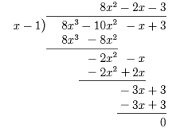
\includegraphics[width=0.5\textwidth]{division}
\end{center}
\item
조립제법을 사용하는 방법
\par
\begin{center}
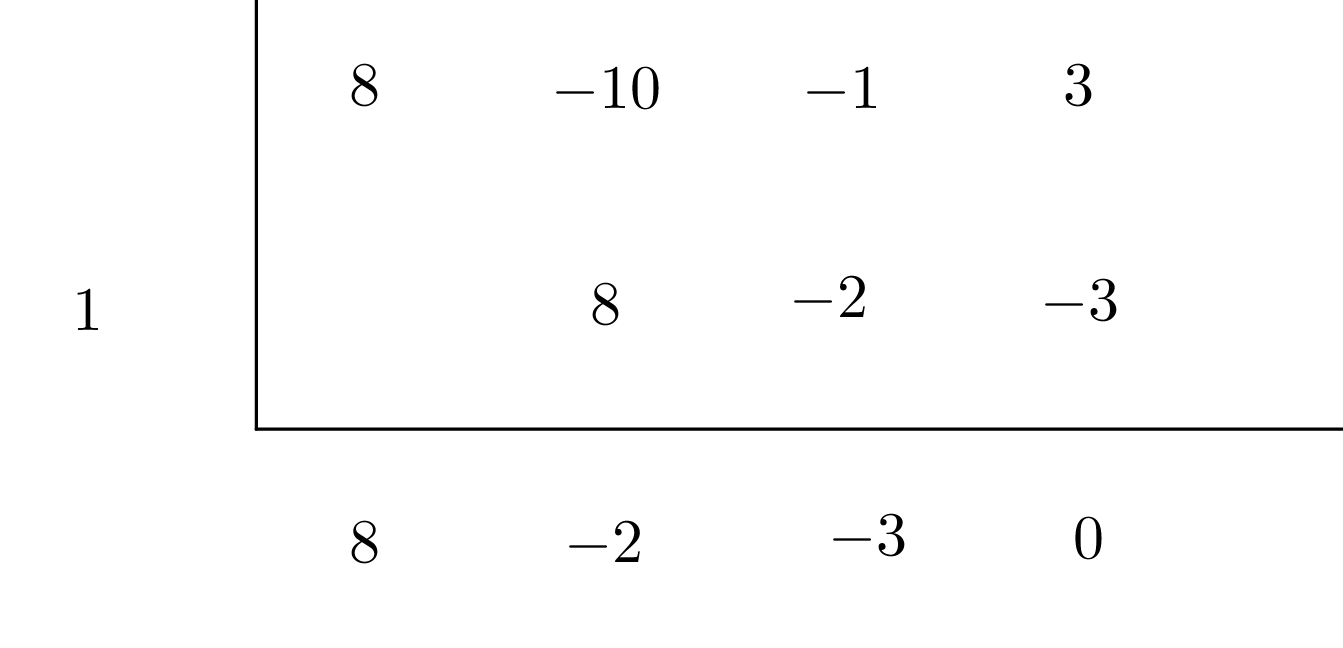
\includegraphics[width=0.5\textwidth]{division_2}
\end{center}
\end{enumerate}
\end{mdframed}
{\par\raggedleft\textbf{몫 : \(8x^2-2x-3\), 나머지 : \(0\)\\
나눗셈 식 : \(2x^3+3x+1=(x+2)(8x^2-2x-3)+0\)
}\par}\bigskip

%
\prob{}
다음 나눗셈의  몫과 나머지를 구하고 나눗셈 식으로 나타내어라.
\begin{enumerate}
\item
\((3x^3-2x^2-3x-5)\div(x-2)\)
\item
\((4x^3+7x^2-12x+3)\div(x+3)\)
\end{enumerate}

%%
\section*{답}

%
\an{2}
\ding{175}

%
\an{4}
\begin{enumerate}
\vspace{-20pt}
\item
\(3x^3+4x^2-x-5\)
\item
\(x^3-3yx^2+2x+4y^3+y\)
\end{enumerate}

%
\an{7}
\vspace{-20pt}
\begin{enumerate}
\item
\(A+B=6x^3-2x-1\)
\item
\(A-B=6x^3+8x^2-5\)
\end{enumerate}

%
\an{9}
(1)\:\:\(a^8\)
\tabto{0.33\textwidth}
(2)\:\:\(-288a^{11}b^{16}c^6\)
\tabto{0.66\textwidth}
(3)\:\:\(a^{lmn}\)\\
(4)\:\:\(\frac{x^7y^9}{z^7}\)
\tabto{0.33\textwidth}
(5)\:\:\(\frac1{p^6q^4}\)
\medskip

%
\an{12}
\begin{enumerate}
\vspace{-20pt}
\item
\(x^3+5x^2+2x-8\)
\item
\(a^3-3a^2b+3ab^2-b^3\)
\item
\(x^3-(a+b+c)x^2+(ab+bc+ca)x-abc\)
\end{enumerate}

%
\an{14}
\begin{enumerate}
\vspace{-20pt}
\item
\(a^2+b^2+c^2-ab-bc-ca\)
\item
\(a^4+a^2b^2+b^4\)
\end{enumerate}

%
\an{19}
\begin{enumerate}
\item
몫 : \(3x^2+4x+5\),\quad 나머지 : \(5\)\\
나눗셈식 : \(3x^3-2x^2-3x-5=(x-2)(3x^2+4x+5)+5\)
\item
몫 : \(4x^2-5x+3\),\quad 나머지 : \(-6\)\\
나눗셈식 : \(4x^3+7x^2-12x+3=(x+3)(4x^2-4x+3)-6\)
\end{enumerate}


\end{document}